%\section{Evaluation: Scalability of the Current Implementation}\label{sec:evaluation}
\section{\textbf{Evaluation }}\label{sec:evaluation} 


Wireshark and Iperf, as open-source tools, are employed to take measurements and read the values to get the best tolerable results. 
Wireshark is a free open-source network packet analyzer. It is used to capture data packets and display the most accurate details achievable about them. Similarly, Iperf is an open-source tool for active measurements of the peak possible bandwidth on IP networks. Besides, it supports harmonizing many factors related to timing and protocols ( Transmission Control Protocol (TCP), User Datagram Protocol (UDP), Stream Control Transmission Protocol (SCTP) with IPv4 and IPv6)\cite{iperf2021}.
Other significant advantages are that Iperf can be utilized in two forms: server and client modes. In addition, it supports End-to-end (E2E) testing and affords a throughput measurement report between the two ends in one or both directions. It handles both data streams: Transmission Control Protocol (TCP) or User Datagram Protocol (UDP). The primary target of (E2E) testing is to examine the end user's activity by simulating the real user scenario and validating the system under test and its elements for combination and data integrity. It is beneficial for analyzing network traffic in real-time.
Figure \textbf{\ref{fig:5gcn-deployment-gnbsim}} presents the Wireshark user interface. We start the 5GC Network components: NRF, Mysql, AMF, SMF, and SPGWU. Then we capture packets on the docker-compose host as shown in the bottom section. The initial data exchanges between the core network components are evident here.
Furthermore, capturing these packets is fundamental, allowing us to see the expected exchange between SMF, RNF, and UPF. SMF can discover UPF using the service discovery feature of NRF. The core network should be correctly configured and healthy, as displayed in figure
\textbf{\ref{fig:corenetwork_are_healthy}}. The completely evaluation process, including taking measurements and monitoring time synchronization, reliability, latency, and determinism, will be explained in detail in the master's paper\cite{openairinterface2014}.
 
 


\begin{figure}
\centering
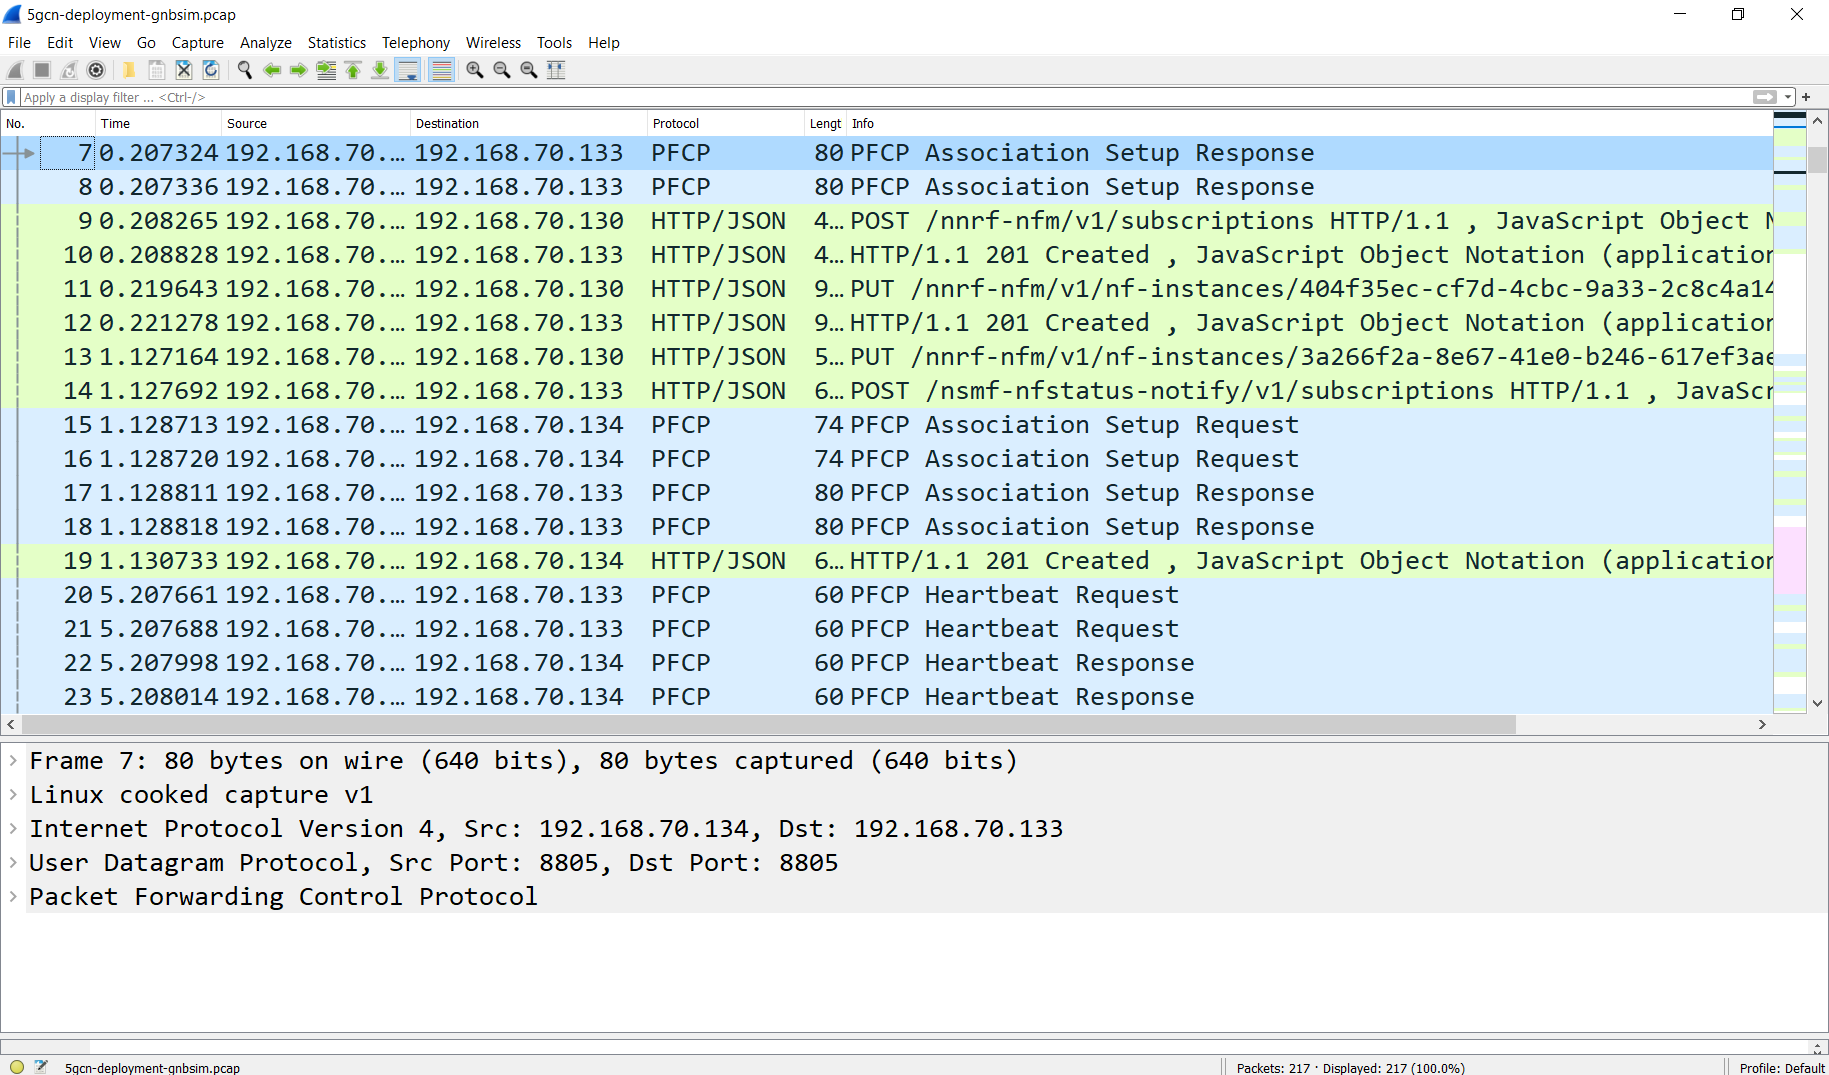
\includegraphics[scale=0.18]{images/5gcn-deployment-gnbsim.png}
\caption{5GC Network Deployment gNBsim \cite{openairinterface2014}}
\label{fig:5gcn-deployment-gnbsim}
\end{figure}






\begin{figure}
\centering
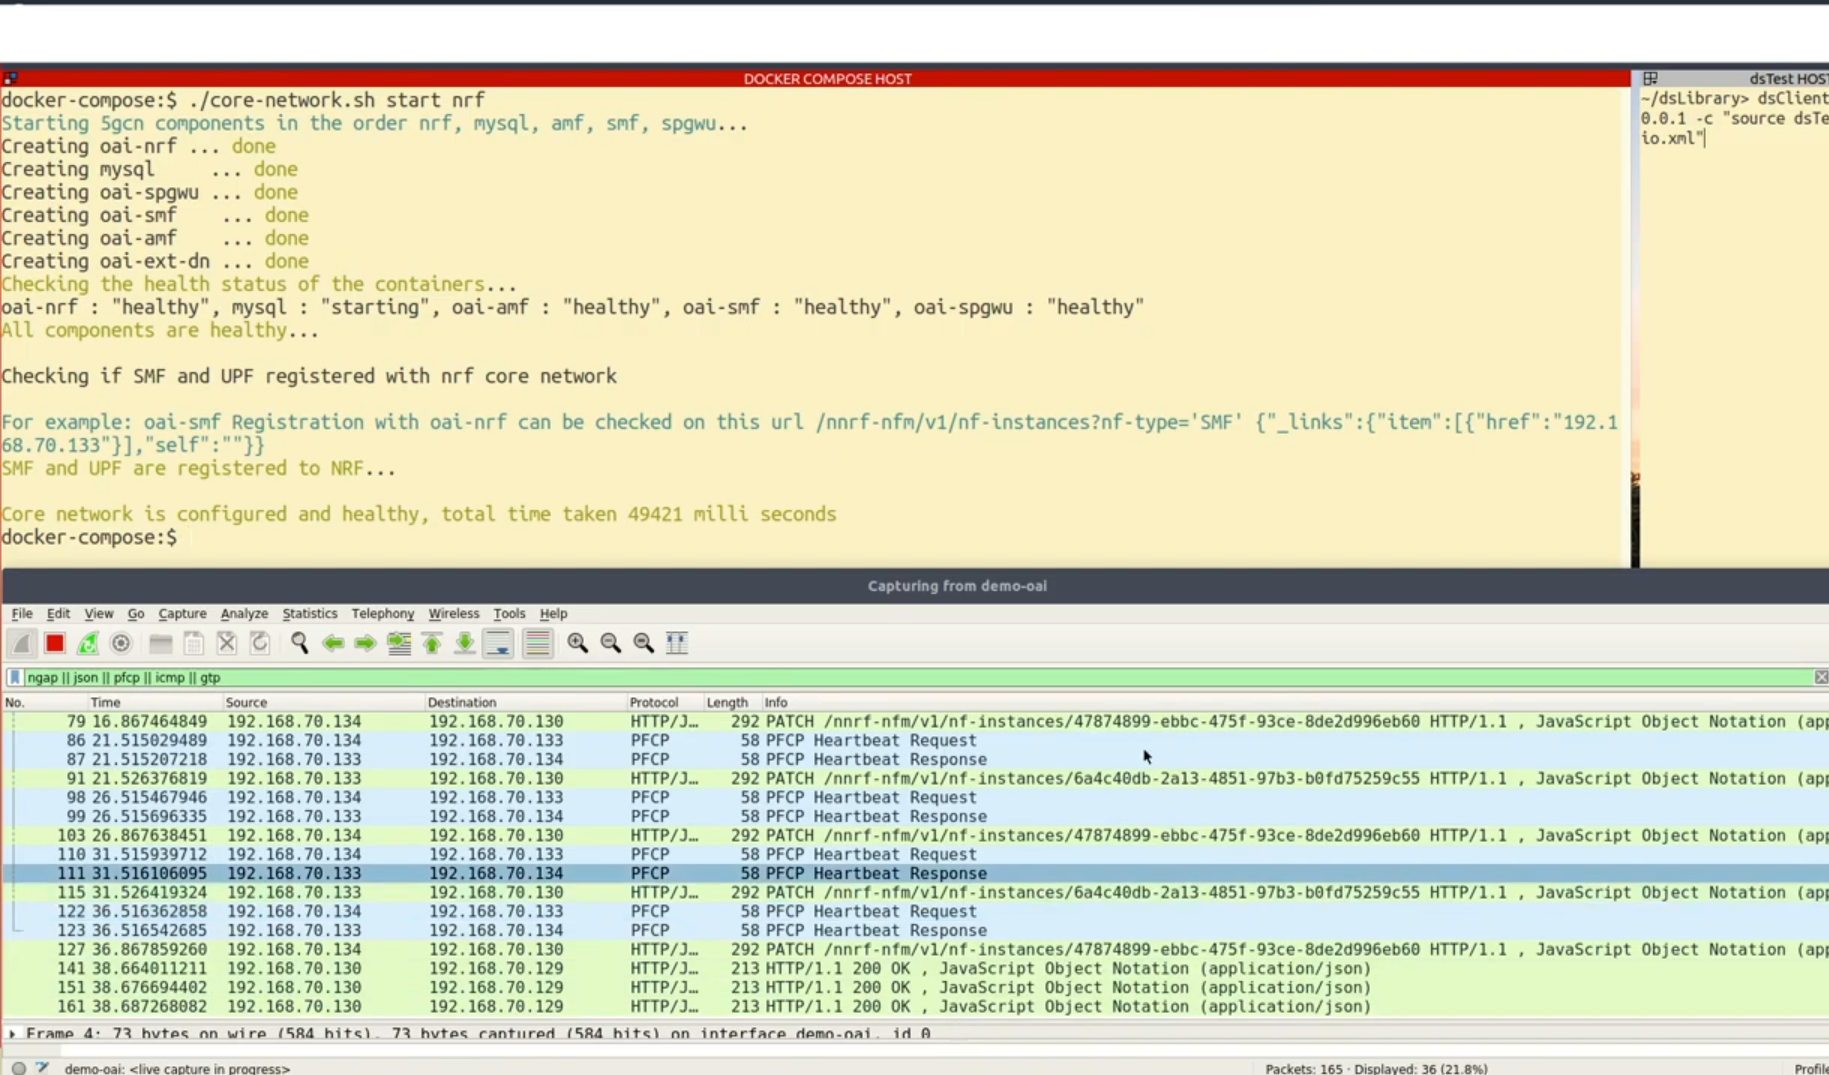
\includegraphics[scale=0.18]{images/corenetwork_are_healthy.png}
\caption{Core Network are healthy and configured \cite{openairinterface2014}.}
\label{fig:corenetwork_are_healthy}
\end{figure}


 

%mmm\subsection{Comparative analysis of Open Source 5G Core implementations (NextEPC, Free5GC, ...) } 
 


% MMM \subsection{Use cases of this Architecture}\label{Use cases of this Architecture}


%-------------------------------------------------------------------------------
%Evaluation: How does it really work in practice? Provide real or simulated
%performance metrics, end-user studies, mention external technology adoptors,
%if any, etc.

%This section presents the detailed results you have obtained. If the paper
%is theoretical, you might want to show curves obtained from your equations.
%If the paper is experimental, you will be presenting curves showing the
%measurement results. In order to choose the proper curves to present, you
%must first be clear what point you are trying to convey to the reader. The 
%curves can then be chosen to illustrate this point. Whether your paper is
%theoretical or experimental, you must provide a careful interpretation of
%what your results mean and why they behave as they do.
%-------------------------------------------------------------------------------
% This section presents the detailed results obtained. It contains the results
% obtained from the analytical model, the emulations and the simulations realized
% as well as the interpretation and discussion of them. 
%-------------------------------------------------------------------------------
% The goals of the study,
% The system boundaries
% System services and possible outcomes
% Selected performance metrics
% System and workload parameters
% Factors and their values
% Evaluation techniques
% Selected workload
% Design of the experiments
% Analysis and interpretation of the data
% Presentation of the results
%------------------------------------------------------------------------------_

%mmm Evaluation: How does it really work in practice? Provide real or simulated performance metrics, end-user studies, mention external technology adopters, if any, and so on.                                %This section presents the detailed results you have obtained. If the paper is theoretical, you might want to show curves obtained from your equations. 
%If the paper is experimental, you will be presenting curves showing the  measurement results. In order to choose the proper curves to present, you must first be clear what point you are trying to convey to the reader. The curves can then be chosen to illustrate this point. Whether your paper is theoretical or experimental, you must provide a careful interpretation of what your results mean and why they behave as they do.

\section{\textbf{Expected Result}}\label{Expected Result}
%\subsection{Study of what is needed}\label{Study of what is needed}
%\subsection{Best effort testbed environment}\label{Best effort testbed environment}


The expected result usually will be:  releasing a signal with 5g logo and uplink or downlink data after turning on the WiFi in all connected mobile phones, the ability to connect a massive number of mobile phones, all phones can watch HD video at the same time. However, the expected result will be limited to the captured packets in Wireshark and Iperf tools because of international health status and costs.
As we previously explained, The initial data exchanges between the core network components are evident At the bottom window of the Wireshark. Additionally, capturing these packets is significant, seeing the expected exchange between SMF, RNF, and UPF. Furthermore, SMF can discover UPF using the service discovery feature of NRF. We can observe intermediary request responses between UPF and SMF. Wireshark shows the signaling process and when UE is accessed, such as registration, authentication, PDU session establishment, an uplink, or downlink GTP packet. Within viewing the AMF log, which showed in figure  \ref{fig:amf_log_user_observed}, we can see that there is already a user Observed.
 

 


\begin{figure}
\centering
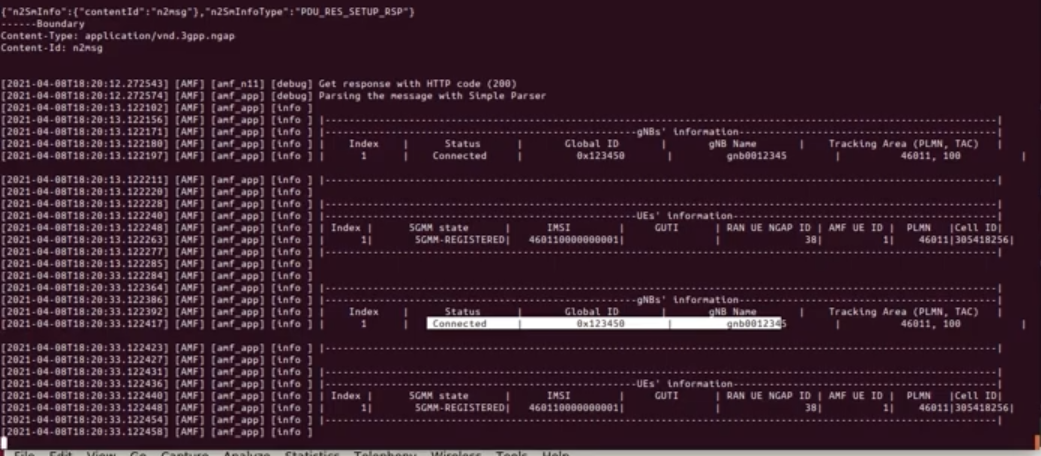
\includegraphics[scale=0.33]{images/amf_log_user_observed.png}
\caption{A user observed in AMF log \cite{openairinterface2014}.}
\label{fig:amf_log_user_observed}
\end{figure}

 
In the SMF log, we can understand that the IP sent by SMF is the same as the phone. 
Nevertheless, it displays data and other session messages. After stopping the 5GC components services, we can see that the phone loses the signal in case of the possibility to use a phone. All the logs file, including 5gcn-deployment-gnbsim.pcap, amf.log, initialmessage.log, smf.log, nrf.log, and spgwu.log will be viewed in the final paper.
   
 